%! TEX program = pdflatex

\documentclass[oneside,solution]{tmpl}

\usepackage[utf8]{inputenc}
\usepackage[english,ukrainian]{babel}
\usepackage{float}

\title{Домашня робота}
\author{Захаров Дмитро}
\studentID{МП-31}
\instructor{Ігнатович С.Ю.}
\date{\today}
\duedate{23:59 30 квітня, 2024}
\assignno{9}
\semester{Весняний семестр 2024}
\mainproblem{Рекурентне логістичне рівняння}

\begin{document}

\maketitle

% \startsolution[print]

\problem{}

\hspace{20px}\textbf{Умова.} Маємо рекурентне рівняння
\begin{equation}
    x_{n+1} = x_n^2 + c
\end{equation}

\begin{enumerate}
    \item Знайдіть нерухомі точки цього відображення, дослідіть їх стійкість.
    \item З'ясуйте, при якому значенні параметра $c$ з'являється стійкий цикл довжини $2$.
    \item Зобразіть павутинну діаграму для рівняння $x_{n+1} = x_n^2 + c$ при якому-небудь цікавому значенні параметра $c$.
    \item Нарисуйте біфуркаційну діаграму для рівняння $x_{n+1} = x_n^2 + c$.
\end{enumerate}

\textbf{Розв'язання.} 

\textbf{Пункт 1.} Нехай маємо відображення $f(x) = x^2 + c$. За означенням, нерухомою точкою є розв'язок рівняння $f(x) = x$, тобто
\begin{equation}
    x^2 - x + c = 0
\end{equation}

Дискримінант $D = 1-4c$, тому при $c \leq \frac{1}{4}$ рівняння буде мати хоч один розв'язок (помітимо, що розглядаємо ми як раз відрізок $c \in [-2, \frac{1}{4}]$). Якщо $c=\frac{1}{4}$ то розв'язком є лише точка $x = \frac{1}{2}$. Якщо ж $c < \frac{1}{4}$, то маємо дві точки
\begin{equation}
    x_1 = \frac{1 + \sqrt{1-4c}}{2}, \; x_2 = \frac{1-\sqrt{1-4c}}{2}
\end{equation}

Для аналізу стійкості, знайдемо похідну відображення. Маємо $f'(x) = 2x$. Підставимо наші дві точки:
\begin{equation}
    f'(x_1) = 1+\sqrt{1-4c}, \; f'(x_2) = 1 - \sqrt{1 - 4c}
\end{equation}

Бачимо, що $f'(x_1) > 1$ для будь-якого $c < \frac{1}{4}$, отже точка нестійка (відштовхує). В свою чергу ситуація з $f'(x_2)$ дещо складніша:
\begin{enumerate}
    \item При $-\frac{1}{4} < c < \frac{1}{4}$ точка стійка, бо $|f'(x_2)| < 1$.
    \item При $0 < c < \frac{1}{4}$ маємо $0 < f'(x_2) < 1$, тому послідовність монотонна.
    \item При $-\frac{1}{4} < c < 0$ маємо $-1 < f'(x_2) < 0$, тому орбіта наближається до $x_2$ з двох боків.
    \item При $c < -\frac{1}{4}$ маємо $f'(x_2) < -1$, тому орбіта стає нестійкою.
\end{enumerate}

Упевнемось у цьому. Запустимо програму нижче:
\begin{lstlisting}[language=Python]
import numpy as np
import matplotlib.pyplot as plt

c = -0.2
f = lambda x: x**2 + c

fig, ax = plt.subplots()
ax.set_aspect('equal', 'box')
ax.grid()

ax.plot([-3, 3], [-3, 3], linestyle='dashed', color='gray')
x = np.linspace(-1.1, 1.1, 100)
ax.plot(x, f(x), linestyle='dashed', color='gray')
ax.set_xlim(-1, 1)
ax.set_ylim(c - 0.1, 1)
plt.axvline(x = (1 - np.sqrt(1 - 4*c)) / 2, linestyle='dashed', color = 'green', label = 'axvline - full height')

x = 0.8
y = f(x)

for _ in range(1, 100):
    z = f(y)
    ax.plot([x,y,y], [y,y,z], color='b', alpha=0.8)
    x, y = y, z
    
plt.savefig('problem_1.pdf')
\end{lstlisting}

На виході отримаємо рис. \ref{fig:1}. Дійсно, як бачимо, наша ``спіраль'' починає накручуватись на точку, що відповідає значенню $\frac{1-\sqrt{1-4c}}{2}$.

\begin{figure}
    \centering
    \includegraphics[width=0.7\textwidth]{images/hw_9/1.pdf}
    \caption{Павутинна діаграма для $c=-0.2$ та $x_0=0.8$. Зеленим пунктиром відмічена лінія $x=\frac{1-\sqrt{1-4c}}{2}$.}
    \label{fig:1}
\end{figure}

\vspace{7.5px}
\textbf{Пункт 2.} Для цього пункту потрібно знайти розв'язок $f(f(x)) = x$ або аналогічно $h(x) := f(f(x)) - x = 0$ -- таке позначення буде нам зручним. Видно, що $f(f(x)) = f(x)^2 + c = (x^2 + c)^2 + c$. Отже:
\begin{equation}
    (x^2 + c)^2 + c = x \iff x^4 + 2cx^2 - x + (c^2 + c) = 0
\end{equation}

Отже $h(x)$ є поліномом 4 ступеня і нам потрібно знайти його нулі. Зазвичай це доволі громіздка задача, але ми можемо викрутитись. По-перше помітимо, що $x_1$ та $x_2$ є корнями $h(x)$. Дійсно,
\begin{equation}
    (x_{1,2}^2+c)^2 + c = x_{1,2}^2 + c = x_{1,2} \implies h(x_{1,2}) = 0
\end{equation}

В такому разі це означає, що $(x-x_1)(x-x_2)=(x^2-x+c) \mid h(x)$, а отже два інших кореня можна знайти з рівняння $h(x)/(x^2-x+c) = 0$, що дає нам:
\begin{equation}
    x^2 + x + (1+c) = 0
\end{equation}

Дискримінант в цьому випадку $D = -3-4c$, тому маємо два додаткових кореня при $c \leq -\frac{3}{4}$. Самі корені це $x_3 = \frac{-1+\sqrt{-3-4c}}{2}$ та $x_4 = \frac{-1-\sqrt{-3-4c}}{2}$. Знайдемо похідну нашого відображення:
\begin{equation}
    f(f(x))' = 4x^3 + 4cx = 4x(x^2 + c)
\end{equation}

Трошки нудні розрахунки показують, що $|d_x f\circ f(x_2)| < 1$ лише при $c \in (-\frac{3}{4}, \frac{1}{4})$, тобто $x_2$ для $c < -\frac{3}{4}$ є нестійкою точкою. Так само для $x_1$, але тут вона ніколи не є стійкою. А ось як $x_3$, так і $x_4$ є стійкими за умови $c \in (-\frac{5}{4}, -\frac{3}{4})$. 

Перевіримо це за допомоги програми нижче:
\begin{lstlisting}[language=Python]
c = -0.85
f = lambda x: x**2 + c

fig, ax = plt.subplots()
ax.set_aspect('equal', 'box')
ax.grid()

x = np.linspace(-1.1, 1.1, 100)
ax.plot([-3, 3], [-3, 3], linestyle='dashed', color='black', alpha=0.3)
ax.plot(x, f(x), linestyle='dashed', color='black', alpha=0.3)
ax.plot(x, f(f(x)), linestyle='dashed', color='black')
ax.set_xlim(-1, 1)
ax.set_ylim(c - 0.1, 1)
plt.axvline(x = (-1-np.sqrt(-3-4*c))/2.0, linestyle='dashed', color = 'green', label = 'axvline - full height')
plt.axvline(x = (-1+np.sqrt(-3-4*c))/2.0, linestyle='dashed', color = 'green', label = 'axvline - full height')

x = -0.35
y = f(x)

# Skipping first 100 iterations
for _ in range(1,100):
    z = f(y)
    x, y = y, z

for _ in range(1,100):
    z = f(y)
    ax.plot([x,y,y], [y,y,z], color='b', alpha=0.8)
    x, y = y, z
    
plt.savefig('problem_2.pdf')
\end{lstlisting}

Результат показано на Рисунку \ref{fig:2}.
\begin{figure}
    \centering
    \includegraphics[width=0.7\textwidth]{images/hw_9/2.pdf}
    \caption{Павутинна діаграма для $c=-0.85$ та $x_0=-0.35$. Зеленим пунктиром відмічені лінії $x=\frac{-1\pm\sqrt{-3-4c}}{2}$.}
    \label{fig:2}
\end{figure}

\textbf{Пункт 3.} Достатньо цікава картинка виходить при $c=-1.87, x_0=0.8$. Результат зображено на Рисунку \ref{fig:3}.
\begin{figure}
    \centering
    \includegraphics[width=0.7\textwidth]{images/hw_9/3.pdf}
    \caption{Павутинна діаграма для $c=-1.87$ та $x_0=0.8$.}
    \label{fig:3}
\end{figure}

\textbf{Пункт 4.} Застосуємо наступну програму:
\begin{lstlisting}[language=Python]
N0 = 200
N = 300
P = 5000
a, b = -2, 0.25

def f(c, x):
    return x**2 + c

fig, ax = plt.subplots()
ax.grid()
r = np.linspace(a, b, P)
x = 0.5 * np.ones((P,))

for _ in range(N0) :
    x = f(r, x)
    
for _ in range(N):
    x = f(r, x)
    ax.plot(r, x, marker ='o', markersize=0.02, color ='blue', linestyle='None')
    
plt.savefig('4.png', dpi=1000)
\end{lstlisting}

Отримаємо Рисунок \ref{fig:4}. Бачимо, що дійсно є точки біфуркації $c=-\frac{3}{4}$ та $c=-\frac{5}{4}$, що ми передбачували до цього.

\begin{figure}
    \centering
    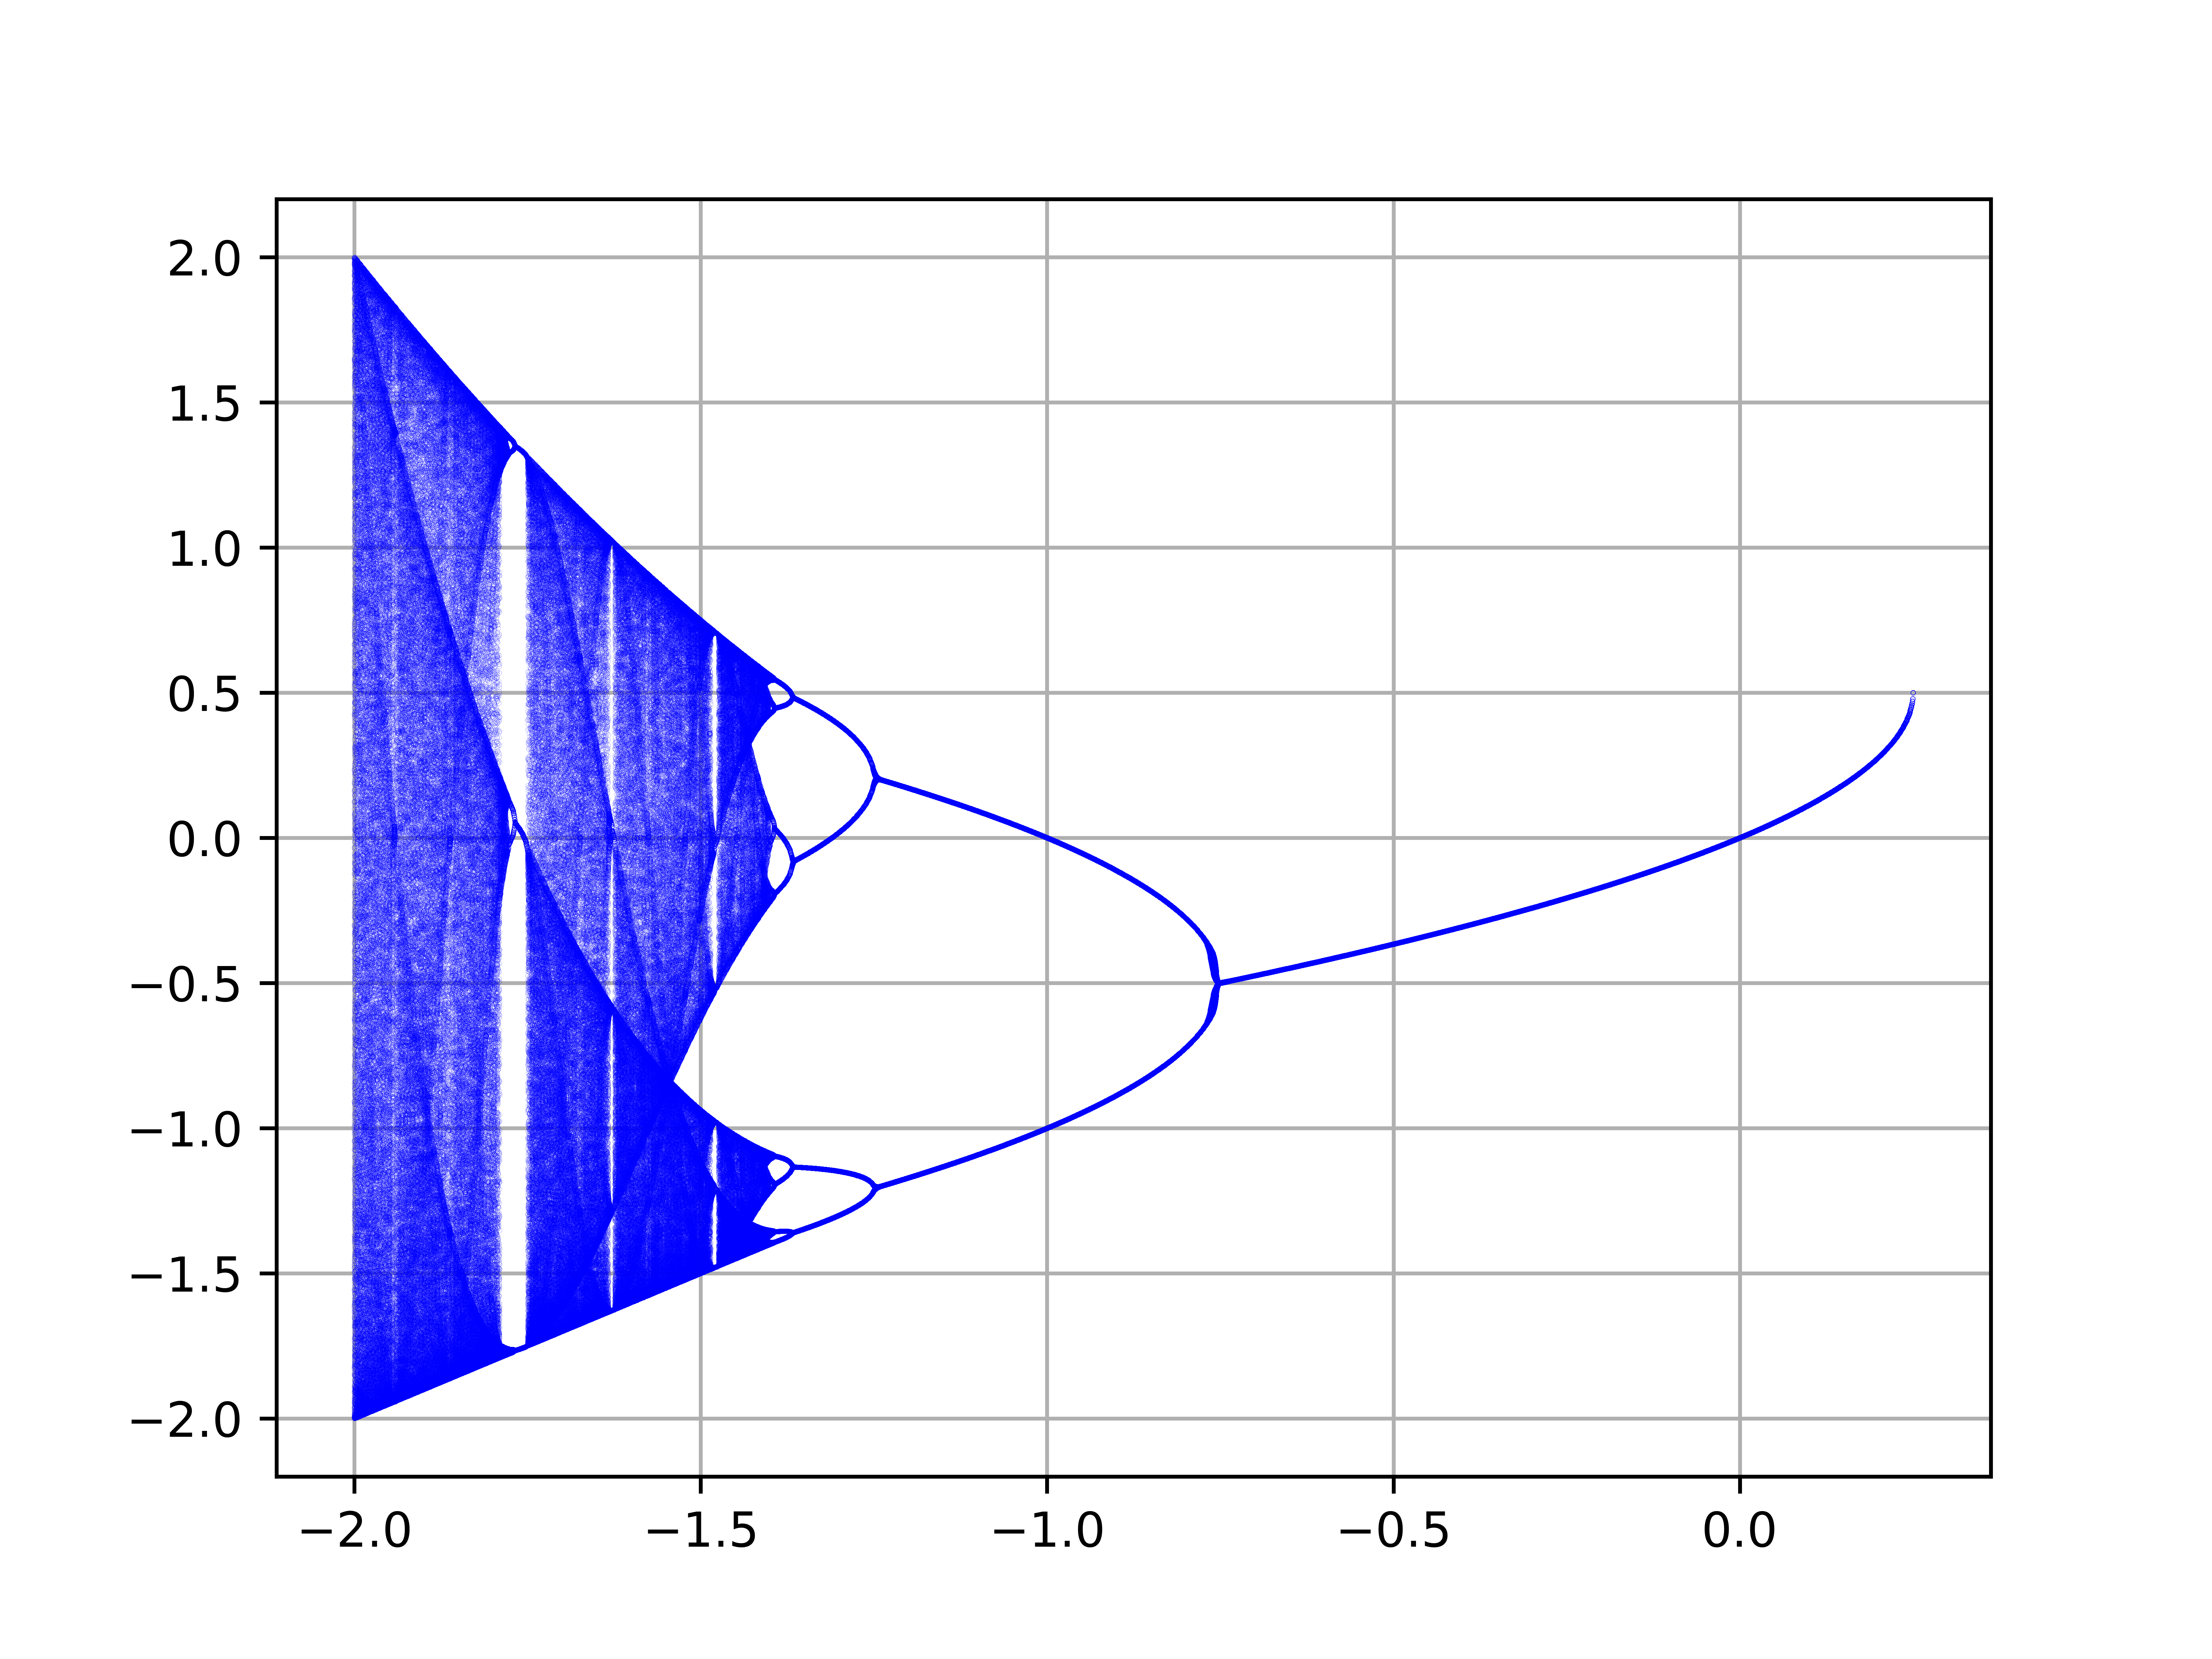
\includegraphics[width=\textwidth]{images/hw_9/4.png}
    \caption{Біфуркаційна діаграма для $x_{n+1}=x_n^2+c$.}
    \label{fig:4}
\end{figure}

\end{document}
